\documentclass[border=16pt]{standalone}
\usepackage[T1]{fontenc}
\usepackage[utf8]{inputenc}
\usepackage{circuitikz}
\usepackage{amsmath,amssymb}
\usetikzlibrary{positioning,calc}
\ctikzset{bipoles/length=1.1cm, font=\small}

% paleta para FONDO BLANCO (imprimible)
\definecolor{tinta}{HTML}{1E293B}
\definecolor{ambar}{HTML}{C2410C}
\definecolor{azul}{HTML}{0E7490}
\definecolor{verde}{HTML}{15803D}
\definecolor{rojo}{HTML}{B91C1C}
\definecolor{gris}{HTML}{6B7280}
\definecolor{panel}{HTML}{F1F5F9}

\begin{document}
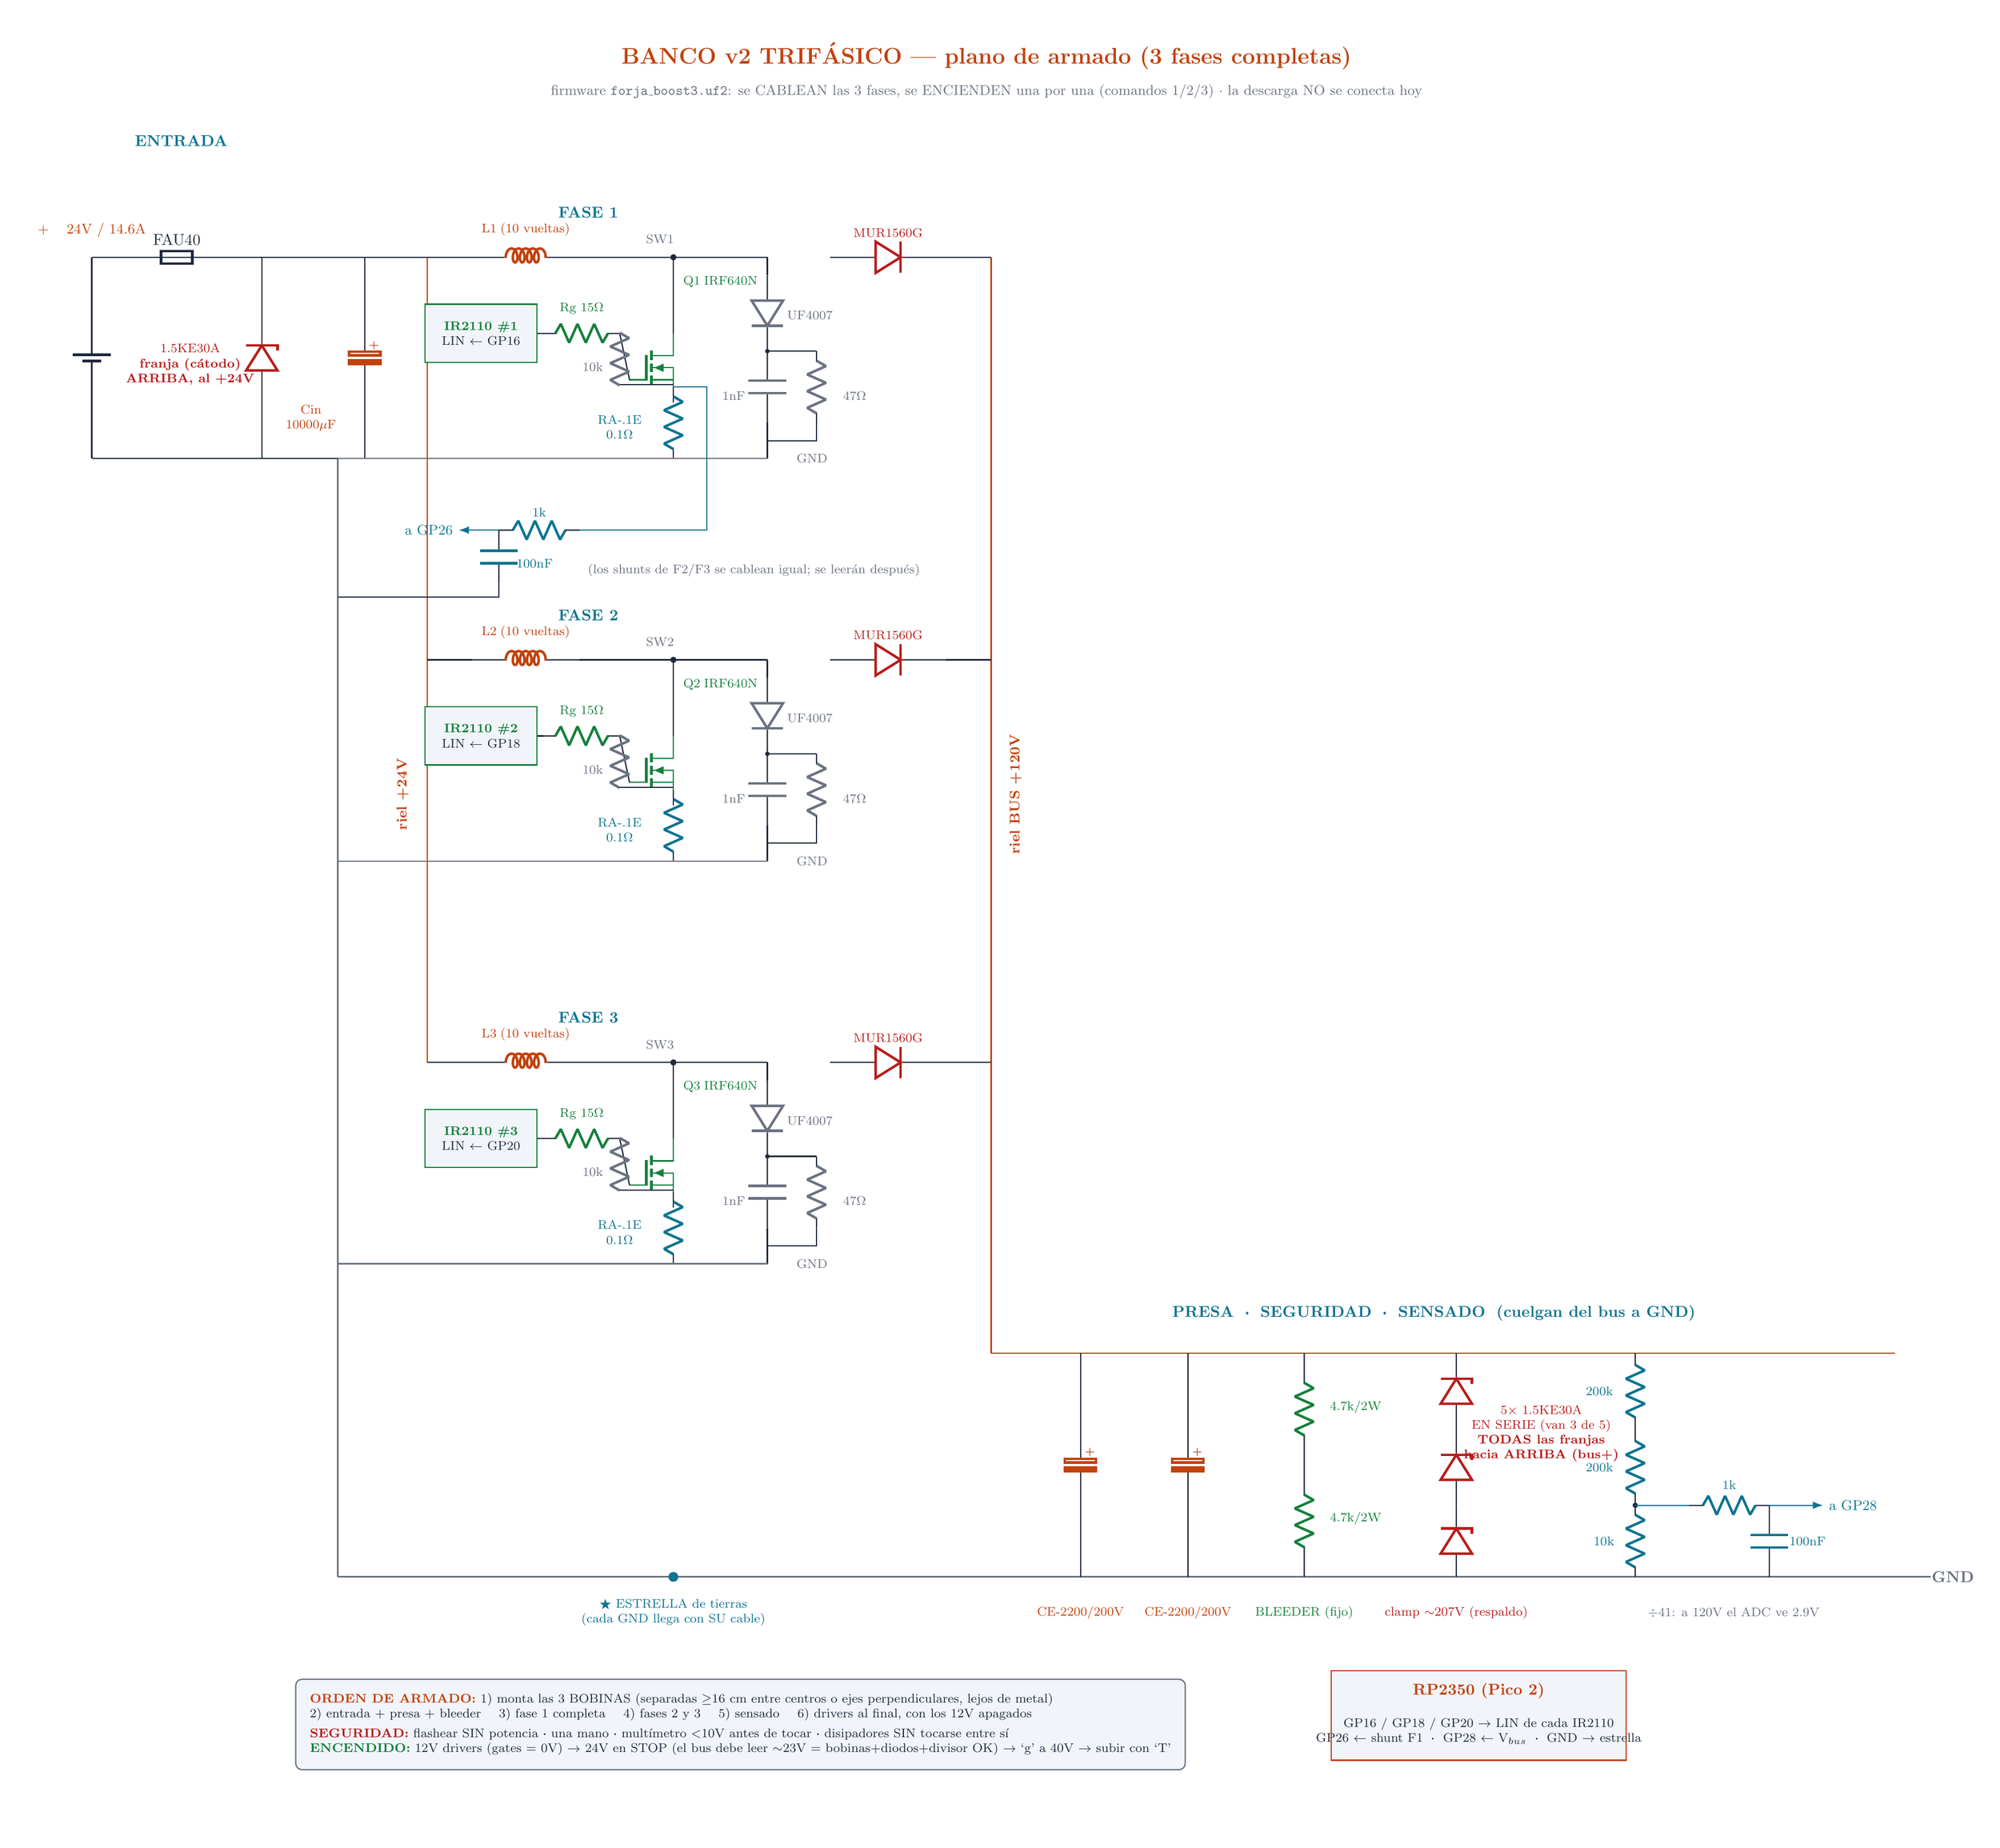
\begin{tikzpicture}[color=tinta, every node/.style={text=tinta}, line width=0.8pt]
\fill[white] (-7.2,-35.2) rectangle (36.8,5.4);

% ===================== TITULO =====================
\node[text=ambar, font=\bfseries\Large] at (14.5,4.5) {BANCO v2 TRIFÁSICO — plano de armado (3 fases completas)};
\node[text=gris, font=\small] at (14.5,3.7) {firmware \texttt{forja\_boost3.uf2}: se CABLEAN las 3 fases, se ENCIENDEN una por una (comandos 1/2/3) · la descarga NO se conecta hoy};

% ===================== ENTRADA (compartida) =====================
\node[text=azul, font=\bfseries] at (-3.5,2.6) {ENTRADA};
\draw (-5.5,0) to[battery1] (-5.5,-4.5);
\node[text=ambar, font=\small] at (-5.5,0.6) {+ \;\; 24V / 14.6A};
\draw (-5.5,-4.5) -- (0,-4.5);
\draw (-5.5,0) -- (-4.5,0);
\draw (-4.5,0) to[fuse, l=\textcolor{tinta}{FAU40}] (-2.7,0);
\draw (-2.7,0) -- (2.0,0);
\draw (-1.7,0) to[empty Zener diode, invert, color=rojo] (-1.7,-4.5);
\node[text=rojo, font=\footnotesize, align=center] at (-3.3,-2.4) {1.5KE30A\\\textbf{franja (cátodo)}\\\textbf{ARRIBA, al +24V}};
\draw (0.6,0) to[ecapacitor, color=ambar] (0.6,-4.5);
\node[text=ambar, font=\footnotesize, align=center] at (-0.6,-3.6) {Cin\\10000$\mu$F};
% rieles
\draw[ambar, line width=1.0pt] (2.0,0) -- (2.0,-18);              % riel +24V
\node[text=ambar, font=\bfseries\small, rotate=90] at (1.45,-12.0) {riel +24V};
\draw[gris, line width=1.0pt] (0,-4.5) -- (0,-29.5);              % bajante GND izquierda
\draw[ambar, line width=1.0pt] (14.6,0) -- (14.6,-24.5);          % riel BUS vertical
\node[text=ambar, font=\bfseries\small, rotate=90] at (15.15,-12.0) {riel BUS +120V};

% ===================== LAS 3 FASES (un renglón cada una) =====================
\foreach \k/\yk/\gpio in {1/0/GP16, 2/-9/GP18, 3/-18/GP20}{
  \node[text=azul, font=\bfseries] at (5.6,\yk+1.0) {FASE \k};
  % bobina
  \draw (2.0,\yk) -- (3.0,\yk);
  \draw (3.0,\yk) to[L, color=ambar] (5.4,\yk);
  \node[text=ambar, font=\footnotesize] at (4.2,\yk+0.62) {L\k\;(10 vueltas)};
  \draw (5.4,\yk) -- (7.5,\yk) coordinate (SW\k);
  \fill[tinta] (7.5,\yk) circle (0.07);
  \node[font=\footnotesize, text=gris] at (7.2,\yk+0.4) {SW\k};
  \draw (7.5,\yk) -- (9.6,\yk);
  % MOSFET
  \node[nigfete, anchor=D, color=verde] (Q\k) at (7.5,\yk-1.7) {};
  \draw (SW\k) -- (Q\k.D);
  \node[text=verde, font=\footnotesize] at (8.55,\yk-0.55) {Q\k\;IRF640N};
  \draw (Q\k.S) -- (7.5,\yk-2.9);
  \draw (7.5,\yk-2.9) to[R, color=azul] (7.5,\yk-4.5);
  \node[text=azul, font=\footnotesize, align=center] at (6.3,\yk-3.8) {RA-.1E\\0.1$\Omega$};
  % gate: Rg + pulldown gate-source + driver
  \draw (Q\k.G) -- (6.3,\yk-1.7);
  \draw (6.3,\yk-1.7) to[R, color=verde] (4.6,\yk-1.7);
  \node[text=verde, font=\footnotesize] at (5.45,\yk-1.15) {Rg 15$\Omega$};
  \draw (6.3,\yk-1.7) to[R, color=gris] (6.3,\yk-2.85);
  \node[text=gris, font=\footnotesize] at (5.7,\yk-2.45) {10k};
  \draw (6.3,\yk-2.85) -- (7.5,\yk-2.85);
  \node[draw=verde, fill=panel, minimum width=2.5cm, minimum height=1.3cm, align=center, font=\footnotesize] (DRV\k) at (3.2,\yk-1.7)
    {\textcolor{verde}{\textbf{IR2110 \#\k}}\\LIN $\leftarrow$ \gpio};
  \draw (DRV\k.east) -- (4.6,\yk-1.7);
  % snubber
  \draw (9.6,\yk) -- (9.6,\yk-0.4);
  \draw (9.6,\yk-0.4) to[D, color=gris] (9.6,\yk-2.1);
  \node[text=gris, font=\footnotesize] at (10.55,\yk-1.3) {UF4007};
  \fill[tinta] (9.6,\yk-2.1) circle (0.05);
  \draw (9.6,\yk-2.1) -- (10.7,\yk-2.1);
  \draw (9.6,\yk-2.1) to[C, color=gris] (9.6,\yk-3.7);
  \node[text=gris, font=\footnotesize] at (8.85,\yk-3.1) {1nF};
  \draw (10.7,\yk-2.1) to[R, color=gris] (10.7,\yk-3.7);
  \node[text=gris, font=\footnotesize] at (11.55,\yk-3.1) {47$\Omega$};
  \draw (10.7,\yk-3.7) -- (10.7,\yk-4.1) -- (9.6,\yk-4.1);
  \draw (9.6,\yk-3.7) -- (9.6,\yk-4.5);
  % diodo al bus
  \draw (11.0,\yk) to[D, color=rojo] (13.6,\yk);
  \node[text=rojo, font=\footnotesize] at (12.3,\yk+0.55) {MUR1560G};
  \draw (13.6,\yk) -- (14.6,\yk);
  % GND local del renglón
  \draw[gris] (0,\yk-4.5) -- (9.6,\yk-4.5);
  \node[text=gris, font=\footnotesize] at (10.6,\yk-4.5) {GND};
}

% sense del shunt F1 -> RC -> GP26 (en el hueco entre renglones)
\draw[azul] (7.5,-2.9) -- (8.25,-2.9) -- (8.25,-6.1) -- (5.4,-6.1);
\draw (5.4,-6.1) to[R, color=azul] (3.6,-6.1);
\node[text=azul, font=\footnotesize] at (4.5,-5.7) {1k};
\draw (3.6,-6.1) to[C, color=azul] (3.6,-7.3);
\node[text=azul, font=\footnotesize] at (4.4,-6.85) {100nF};
\draw (3.6,-7.3) -- (3.6,-7.6) -- (0,-7.6);
\draw[azul,-{Latex}] (3.6,-6.1) -- (2.7,-6.1) node[left, text=azul, font=\small]{a GP26};
\node[text=gris, font=\footnotesize] at (9.3,-7.0) {(los shunts de F2/F3 se cablean igual; se leerán después)};

% ===================== BUS: PRESA + SEGURIDAD + SENSADO =====================
\draw[ambar, line width=1.0pt] (14.6,-24.5) -- (34.8,-24.5);
\node[text=azul, font=\bfseries] at (24.5,-23.6) {PRESA \;·\; SEGURIDAD \;·\; SENSADO \;(cuelgan del bus a GND)};
\draw[gris, line width=1.1pt] (0,-29.5) -- (35.6,-29.5);
\node[text=gris, font=\bfseries] at (36.1,-29.5) {GND};
\fill[azul] (7.5,-29.5) circle (0.11);
\node[text=azul, font=\footnotesize, align=center] at (7.5,-30.3) {$\bigstar$ ESTRELLA de tierras\\(cada GND llega con SU cable)};

\draw (16.6,-24.5) to[ecapacitor, color=ambar] (16.6,-29.5);
\node[text=ambar, font=\footnotesize, align=center] at (16.6,-30.3) {CE-2200/200V};
\draw (19.0,-24.5) to[ecapacitor, color=ambar] (19.0,-29.5);
\node[text=ambar, font=\footnotesize, align=center] at (19.0,-30.3) {CE-2200/200V};
\draw (21.6,-24.5) to[R, color=verde] (21.6,-27.0);
\draw (21.6,-27.0) to[R, color=verde] (21.6,-29.5);
\node[text=verde, font=\footnotesize] at (22.75,-25.7) {4.7k/2W};
\node[text=verde, font=\footnotesize] at (22.75,-28.2) {4.7k/2W};
\node[text=verde, font=\footnotesize, align=center] at (21.6,-30.3) {BLEEDER (fijo)};
\draw (25.0,-24.5) to[empty Zener diode, invert, color=rojo] (25.0,-26.2);
\draw (25.0,-26.2) to[empty Zener diode, invert, color=rojo] (25.0,-27.9);
\draw (25.0,-27.9) to[empty Zener diode, invert, color=rojo] (25.0,-29.5);
\node[text=rojo, font=\footnotesize, align=center] at (26.9,-26.3) {5$\times$ 1.5KE30A\\EN SERIE (van 3 de 5)\\\textbf{TODAS las franjas}\\\textbf{hacia ARRIBA (bus+)}};
\node[text=rojo, font=\footnotesize, align=center] at (25.0,-30.3) {clamp $\sim$207V (respaldo)};
\draw (29.0,-24.5) to[R, color=azul] (29.0,-26.2);
\node[text=azul, font=\footnotesize] at (28.2,-25.35) {200k};
\draw (29.0,-26.2) to[R, color=azul] (29.0,-27.9);
\node[text=azul, font=\footnotesize] at (28.2,-27.05) {200k};
\draw (29.0,-27.9) to[R, color=azul] (29.0,-29.5);
\node[text=azul, font=\footnotesize] at (28.3,-28.7) {10k};
\fill[tinta] (29.0,-27.9) circle (0.06);
\draw[azul] (29.0,-27.9) -- (30.2,-27.9);
\draw (30.2,-27.9) to[R, color=azul] (32.0,-27.9);
\node[text=azul, font=\footnotesize] at (31.1,-27.45) {1k};
\draw (32.0,-27.9) to[C, color=azul] (32.0,-29.5);
\node[text=azul, font=\footnotesize] at (32.85,-28.7) {100nF};
\draw[azul,-{Latex}] (32.0,-27.9) -- (33.2,-27.9) node[right, text=azul, font=\small]{a GP28};
\node[text=gris, font=\footnotesize, align=center] at (31.2,-30.3) {$\div$41: a 120V el ADC ve 2.9V};

% ===================== PICO + NOTAS =====================
\node[draw=ambar, fill=panel, minimum width=6.6cm, minimum height=2.0cm, align=center] (PICO) at (25.5,-32.6) {};
\node[text=ambar, font=\bfseries] at (25.5,-32.05) {RP2350 (Pico 2)};
\node[text=tinta, font=\footnotesize, align=center] at (25.5,-32.95)
  {GP16 / GP18 / GP20 $\to$ LIN de cada IR2110\\GP26 $\leftarrow$ shunt F1 \;·\; GP28 $\leftarrow$ V$_{bus}$ \;·\; GND $\to$ estrella};

\node[draw=gris, fill=panel, rounded corners, align=left, inner sep=9pt, font=\footnotesize, text=tinta] at (9.0,-32.8)
 {\textcolor{ambar}{\textbf{ORDEN DE ARMADO:}} 1) monta las 3 BOBINAS (separadas $\geq$16 cm entre centros o ejes perpendiculares, lejos de metal)\\
  2) entrada + presa + bleeder \quad 3) fase 1 completa \quad 4) fases 2 y 3 \quad 5) sensado \quad 6) drivers al final, con los 12V apagados\\[3pt]
  \textcolor{rojo}{\textbf{SEGURIDAD:}} flashear SIN potencia · una mano · multímetro $<$10V antes de tocar · disipadores SIN tocarse entre sí\\
  \textcolor{verde}{\textbf{ENCENDIDO:}} 12V drivers (gates = 0V) $\to$ 24V en STOP (el bus debe leer $\sim$23V = bobinas+diodos+divisor OK) $\to$ `g' a 40V $\to$ subir con `T'};

\end{tikzpicture}
\end{document}
